\begin{theorem}[12.2]\label{12.2}
    $E(\C)$~--- банахово, $A \in K(E), \lambda \in \C, \lambda \neq 0$. Тогда $\dim \ker A_\lambda < \infty$
\end{theorem}

\begin{proof}
    Покажем, что единичная сфера в $\ker A_\lambda$~--- предкомпакт. Посмотрим на языке последовательностей
    \[ 
    \forall \{x_n \} \subset \ker A_\lambda:
    \begin{cases}
    \|x_n\| = 1, \text{ (на сфере) } \forall n\\
    A_{\lambda} x_n = 0
    \end{cases}
    \]
    Покажем, что из $\{x_n\}$ можно выделить сходящуюся подпоследовательность.
    $A[\{x_n\}]$~--- предкомпакт (так как $A$~--- компактный оператор), следовательно,
    по~\nameref{thm3.2} существует сходящаяся подпоследовательность $A_\lambda x_{n_k} = 0 \Longleftrightarrow A x_{n_k} = \lambda x_{n_k} \to y \in \overline{A[\{x_n\}]}$.

    \[\lambda x_{n_k} \to y \lra x_{n_k} \to \frac{1}{\lambda} y \implies Ax_{n_k} \to \frac{1}{\lambda} Ay\]

    Откуда получаем, что $Ay = \lambda y$ (единственность предела), а это значит, что $y \in \ker A_\lambda$.
\end{proof}

\begin{theorem}[12.3]\label{12.3}
$E(\C)$~--- банахово пространство, $A$~--- компактный оператор на $E$. Тогда
$\forall \delta > 0$ вне круга $\{ |\lambda| \leqslant \delta \}$ может лежать лишь конечное число собственных значений оператора $A$.

\begin{figure}[H]
    \centering
    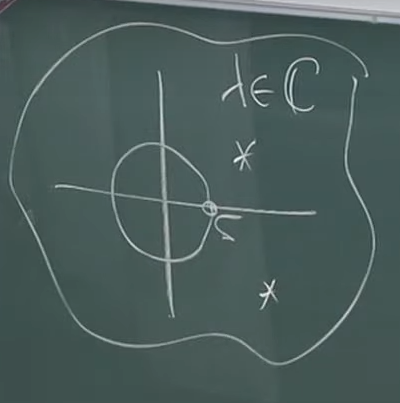
\includegraphics[width=0.25\textwidth]{images/6_2_1.png}
\end{figure}
\end{theorem}

\begin{unnecessary}
\begin{example}
Пусть оператор в $l_2$ задаётся матрицей
$
\begin{pmatrix}
1 \\
_ & 0 \\
_ & _ & \frac{1}{2} \\
_ & _ & _ & 0 \\
_ & _ & _ & _ & \frac{1}{3} \\
_ & _ & _ & _ & _ & \ddots
\end{pmatrix}
$

Это компактный оператор, у которого $0$~--- собственное значение бесконечной кратности.
\end{example}
\end{unnecessary}

\begin{proof}
    Доказательство проведем для случая, когда $E$~--- гильбертово пространство, а $A$~--- компактный самосопряжённый оператор. 

    Предположим противное. $\exists \delta_0$, что вне соответствующего круга $\{|\lambda| < \delta_0\}$ находится бесконечно много собственных значений оператора $A$. Выберем последовательность $\lambda_n$, из этого бесконечного множества. 
    Каждому $\lambda_n$ сопоставлен хотя бы один собственный вектор $e_n$. Тогда из самосопряжённости оператора следует, что при $\lambda_n \neq \lambda_m$ выполнено $(e_n, e_m) = 0$. Отнормируем все $e_n$. 
    Следовательно, $A[\{e_n\}]$~--- предкомпактное множество (это эквивалентно вполне ограниченности).
    Покажем, что это не так. В самом деле, 
    \[\|Ae_n - Ae_m\|^2 = |\lambda_n|^2 + |\lambda_m|^2 > 2 \delta_0^2\]
    Отсюда следует, что $A[\{e_n\}]$~--- не вполне ограничено. Противоречие.
\end{proof}

\begin{lemmanote}
    В общем случае можно несложно доказать через теорему о почти перпендикуляре, но сейчас просто знакомимся с полезными приёмами.
\end{lemmanote}

\begin{corollary}[из теорем \nameref{12.2} и \nameref{12.3}]
    \(\)
    \begin{enumerate}
        \item 
        \(
        \sum \limits_{|\lambda| > \delta > 0} \dim \ker A_{\lambda} < \infty
        \) (конечная сумма конечных размерностей)

        \item $\sigma_p(A)$~--- не более, чем счётное множество (нумеруем круги, вне каждого конечное множества, т.е. можем занумеровать мир ненулевых собственных значений)
    \end{enumerate}
\end{corollary}